\documentclass{article}
\usepackage[margin=1in]{geometry}
\usepackage{graphicx}
\graphicspath{ {./images/} }
\usepackage{hyperref}
\usepackage[parfill]{parskip}
\setlength\parindent{0pt}
\renewcommand{\baselinestretch}{1.5}

\usepackage{amsmath}
\frenchspacing

\title{Ninnion: The Observer's Operation Manual}
\author{CTMO}
\date{v 3020-02-24}

% Contributing authors
%	Richard Camuccio
%	Elizabeth Caputa
%	Moises Castillo
%
% Contributing observers
%   Karina Hernandez
%   Victor Hugo Rangel
%   Tanya Llanas
%   Abigail Martinez
%   Wendy Mendoza
%   Ivan Morado
%   Martell Valencia
%
% Initial version: 2019-07-03

\begin{document}
	
	\maketitle
	
	\begin{figure}[b]
		\centering
		
\includegraphics[scale=0.2]{CTMO_transparent.png}
	\end{figure}
	
	\newpage
	\tableofcontents
	
	\newpage
	\section{Planning an Observation}
	
		Planning an observation requires a few critical steps that should be completed before arriving at the observatory. Entering the observatory with an observation strategy and understanding of the sky conditions is crucial for completing a scientific observation.
	
		\subsection{Check the weather and sky conditions}
	
			\begin{enumerate}
	
				\item Check sunset. It's advised that you choose the beginning of your critical scientific data run to be no earlier than astronomical twilight. Astronomical twilight occurs when the Sun is 18 degrees below the local horizon. In Brownsville, during the summer, astronomical twilight occurs roughly 1.5 hours after sunset. You can certainly observe before this time, during civil or nautical twilight, but extinction by sunlight will be much more significant.
			
				\begin{figure}[h]
					\centering
					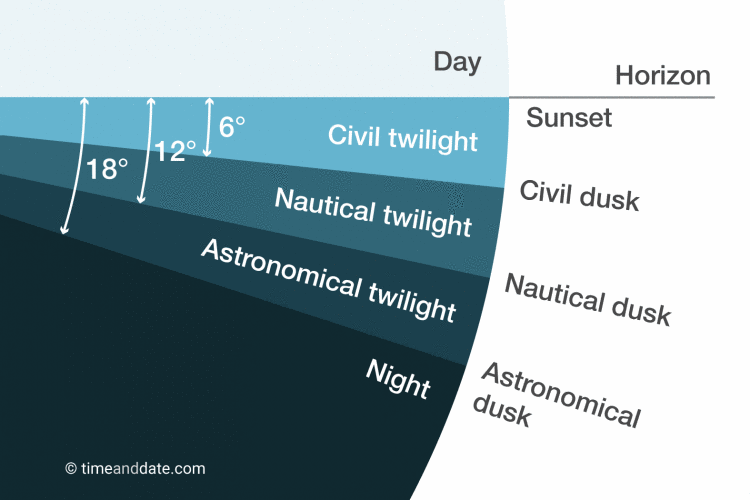
\includegraphics[scale=0.5]{twilight-phases-dusk.png}
				\end{figure}
	
				\item Check forecast. Visit the \href{https://www.weather.gov}{National Weather Service}.
		
				\begin{figure}[h]
					\centering
					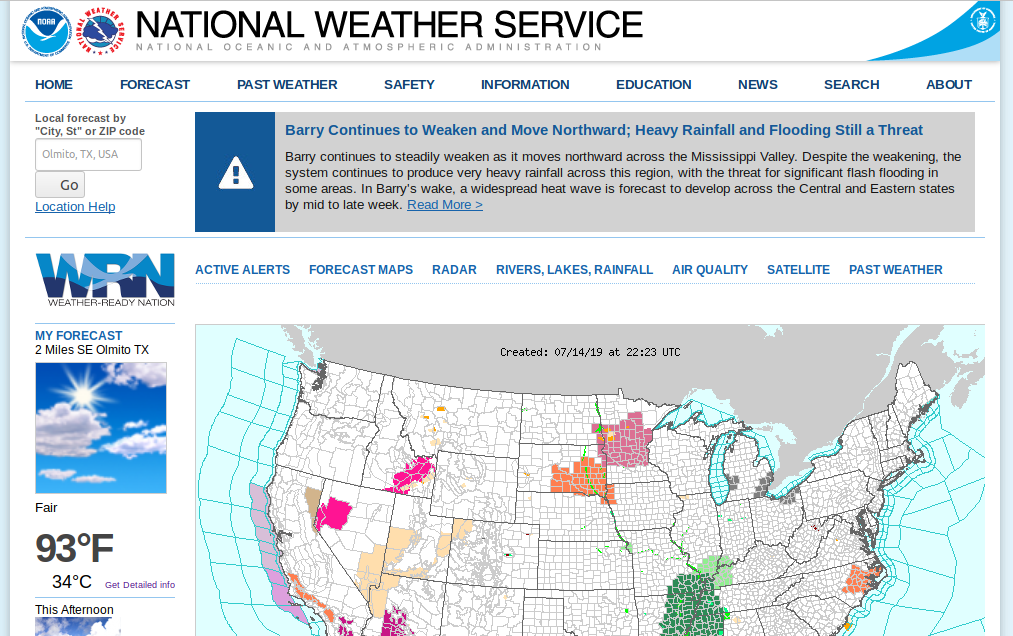
\includegraphics[scale=0.2]{nws.png}
				\end{figure}
			
				\begin{enumerate}
		
					\item At the top left, search and select the location \texttt{Olmito, TX, USA}. This action will take you to a new page with the forecast for Olmito.		
		
					\item Scroll down the new page to the section titled \texttt{Detailed Forecast}.
		
					\begin{figure}[h]
						\centering
						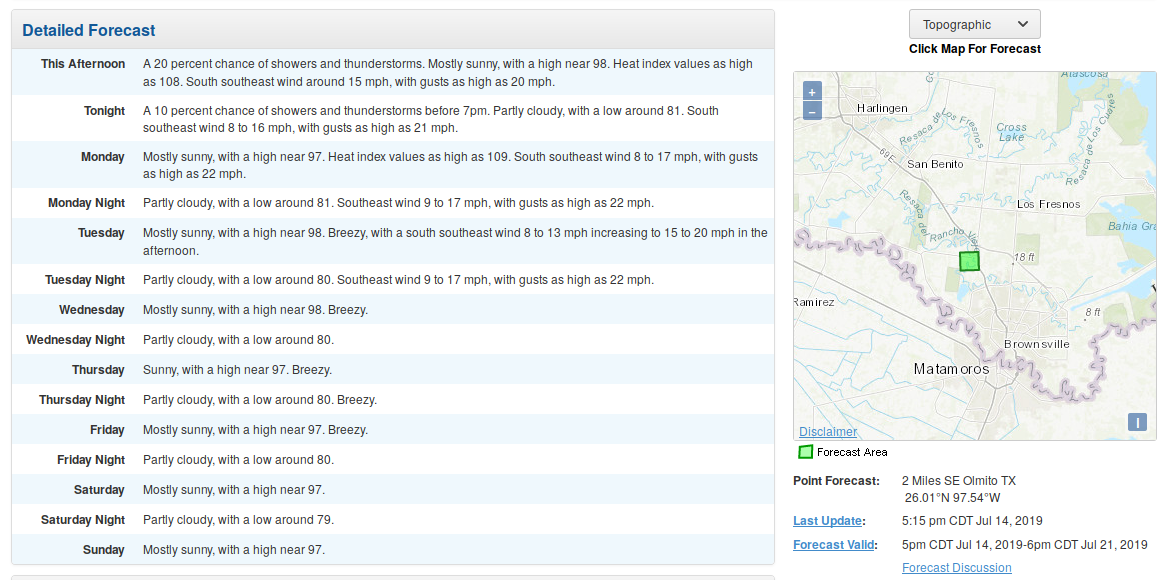
\includegraphics[scale=0.2]{detailed_forecast.png}
					\end{figure}
	
					\item To the right of this you will see a map. Find the approximate location of Resaca de la Palma State Park and click it on the map. The page will reload. You should see the green square highlighting the region you just clicked. This action will reload the page. Scroll back down to the map to confirm the spot you clicked is now highlighted by the square.
		
					\begin{figure}[h]
						\centering
						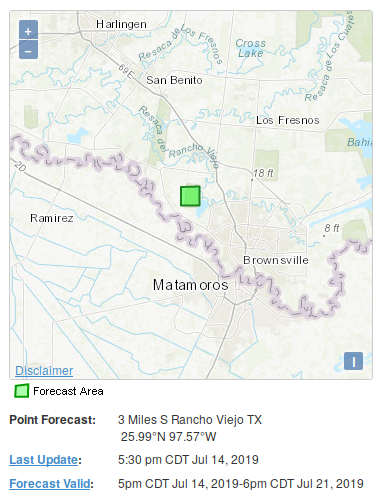
\includegraphics[scale=0.3]{green_square.png}
					\end{figure}
		
					\item Immediately below this, click the graph titled \texttt{Hourly Weather Forecast}. This action takes you to a new page with the forecast in graphical form of the location you clicked. This page is extremely useful and, hence, it is recommended to bookmark this page for future reference.
		
					\begin{figure}[h]
						\centering
						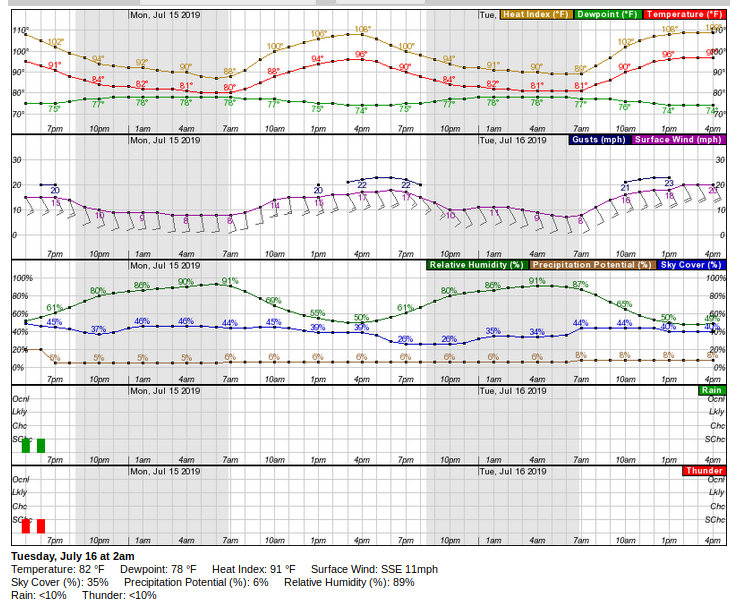
\includegraphics[scale=0.3]{graph.png}
					\end{figure}
				
				\end{enumerate}
			
				\item Check the Moon. Using Stellarium, check to see the phase and position of the Moon during the course of the night. Moonlight significantly interferes with photometric precision. You'll want to make sure your targets are far enough away from the Moon so as not to affect your exposures.
				
				\end{enumerate}
	
		\subsection{Identify your target}
		
			\begin{enumerate}
				
				\item What are the coordinates of your object? Object coordinates are typically expressed in RA (\texttt{hh:mm:ss.ssss}) and Dec (\texttt{$\pm$dd:mm:ss.ssss}) in the J2000 epoch.
				
				\item Check the altitude range over your expected observation time. For accurate photometry, you want to make sure your object is above 30 degrees in altitude. It's useful to visualize the path of the object in the sky ahead of time, using planetarium software like Stellarium.
				
				\item Obtain a reference field for your night. Using Stellarium or any optical image database online like \href{http://simbad.u-strasbg.fr/simbad/}{SIMBAD}, you should find a visual estimation of what your telescope will be pointing
				
				\item Determine suitable reference stars. Make sure they aren't variable stars and that their color indices are similar to your target object.
				
			\end{enumerate}
			
		\subsection{Plan your observing strategy}
		
			\begin{enumerate}
			
				\item What's your strategy?
				
				\begin{enumerate}
					
					\item Do you have a list of targets that you want to observe throughout the night?
					
					\item Are you tracking a single object?
					
					\item Does the object move with proper motion or sidereal motion?
					
				\end{enumerate}
				
				\item If you're planning to observe multiple objects, like a selection of galaxies, then you want to observe the galaxies that are scheduled to set first. That way you can observe the most amount of galaxies on your list at a suitable airmass coefficient.
				
				\item If you're planning to observe a single target over time, then you'll need to plan the exposure time and cadence of your image sequence. This answer will depend on the nature of your target.
				
				\begin{enumerate}
					
					\item Asteroids move with proper motion and can have a wide range of velocities.
					
					\item Exoplanet transits can be quite faint and are at a fixed point in time.
					
					\item Variable stars have a wide variety of periods and magnitude changes.
					
				\end{enumerate}
			
			\end{enumerate}
		
	\newpage
	\section{Starting Up}
	
		\subsection{Entry and Power Up}
		
			\begin{enumerate}
		
				\item Remove padlocks from the hatch. Bring padlocks inside.
		
				\item Turn on the lights. Use the switch on the right side entering the dome.
			
				\item Message the team that the dome has been opened.
	
				\item Turn on all circuit breakers 1-12. Breakers 2, 7, and 11 should always remain ON.
				
				\item Turn on the UPS battery backup. This is the slim, tall box on the table to the immediate left of the breaker box. Turn on using the center power button. After a beep and some warming up, the information screen should indicate the battery is running on the power line rather than on the battery.
		
				\item Turn on the AC unit on the wall.
	
				\item Turn on Atlas. Grub should automatically boot Windows. Turn on the monitor.
		
			\end{enumerate}
		
		\subsection{Open Shutter Window}
		
			\begin{enumerate}

				\item Unplug the battery charger from the wall outlet.
				
				\item Remove the charger from the battery. First remove the RED leads from the RED (+) terminal on the battery. Then remove the BLACK lead from the BLACK (-) terminal on the battery.
			
				\item Remove the charger from the wall and place it safely on the floor.
	
				\item Connect the BLACK motor cable to the BLACK (-) terminal on the battery.
			
				\item Connect the RED motor cable to the RED (+) terminal on the battery.
			
				\item Press and hold \texttt{OPEN} on the shutter controller. Open until the white rubber lip of the shutter window is coincident with the blue metal bar near zenith.
				
			\end{enumerate}
		
		\subsection{Open Shutter Door}
			
			\begin{enumerate}
				
				\item Undo the rope and let down the shutter door. It is normal for the rope to stretch diagonally across the shutter door opening.
				
			\end{enumerate}
		
		\subsection{Prepare Telescope}
		
			\begin{enumerate}
				
				\item Slide the light shroud up toward the front of the optical tube assembly (OTA).
			
				\item Remove the cloth cover from the secondary mirror.
			
				\item Remove the plastic shower cap 
			
				\item Remove the round plastic lid from the primary aperture.
			
				\item Slide the light shroud back down to completely enclose the OTA.
	
				\item Check that the RA and Dec brakes are removed.
			
				\item Turn on the mount.
				
			\end{enumerate}
		
		\subsection{Connect to EFA Kit}
		
			\begin{enumerate}
				
				\item Open PWI3. Verify the computer established connection to the electronic focus assembly (EFA). The EFA should connect automatically to the computer and begin cooling the OTA and primary mirror. You should hear the fans turn on.
				
				\item Click the \texttt{Temperature} tab on the right in PWI3. Record the ambient temperature given by the display.
								
			\end{enumerate}
		
		\subsection{Prepare Camera}
		
			\begin{enumerate}
				
				\item Open MaxIm DL.
							
				\item Connect to camera. Under \texttt{View}, open the \texttt{Camera Control Window}. Select \texttt{Setup} and then \texttt{Connect} to enable computer connection to the camera.
				
				\item Cool camera. Click \texttt{Cooler} and enter the set point. It is advisable to limit the initial set point to no more than 40 degrees C relative to the ambient temperature to avoid over-straining the thermoelectic coolers. For example, if the ambient temperature is 30 degrees C, then the set point should be no less than -10 degrees C.
				
				\item Under \texttt{Connect} select \texttt{On} to begin cooling the camera. The cooler power should not exceed 80\% during operation. If you find that the initial set point can be safely lowered more than the initial set point, you may do so in intervals until a sustained cooler power of 80\% is reached.
				
			\end{enumerate}
		
		\subsection{Connect to Mount}
		
			\begin{enumerate}
								
				\item Open PWI4. Click \texttt{Connect} at the top left of the window.
				
				\item Click \texttt{Enable RA} and \texttt{Enable Dec} under \texttt{Connect}.
	
				\item Make sure the area around the telescope is completely clear.
	
				\item Select \texttt{Commands} and then click \texttt{Home mount}. The telescope will slew and locate its reference encoders.
				
				\item Once the telescope has stopped moving, you are ready to observe!
							
			\end{enumerate}
		
	\newpage
	\section{Observing}
	
	\subsection{Set up directory structure}
	
		\begin{enumerate}
			
			\item Under \texttt{C:\textbackslash Documents\textbackslash Observations} create a directory with the evening date in the format \texttt{yyyy-mm-dd}.
			
			\item Under the newly-made directory, create a directory called \texttt{dark}, a directory called \texttt{flat}, and a directory for each of your targets by name (e.g. for target exoplanet system HAT-P-7 the directory would be something like \texttt{hatp7}).
			
		\end{enumerate}
	
	\subsection{Set up autosave routine}
		
		Note that if you're picking multiple targets, you can either set up multiple autosaves or use the \texttt{Single} exposure option to manually expose each target.
		
		\begin{enumerate}
			
			\item In MaxIm DL, in the \texttt{Camera Control} window, under the \texttt{Expose} tab, click the \texttt{Autosave} button. A new window should appear called \texttt{Autosave Setup}.
			
			\item In the \texttt{Autosave Setup} window, set \texttt{Autosave Filename} to the name of your target.
			
			\item Make sure \texttt{Slot 1} is selected. Frame \texttt{Type} will be \texttt{Light}. Set your \texttt{Exposure}, \texttt{Binning}, and the number of exposures or \texttt{Repeat}.
			
			\item Select \texttt{Options} and \texttt{Set Image Save Path...}. Under \texttt{Documents}, \texttt{Observations}, create a new directory with the current date (in \texttt{yyyy-mm-dd} format). Then, under this new directory, create a new subdirectory with the name of your target. Click \texttt{OK} to close this window.
			
			\item Finally, in the \texttt{Autosave Setup} window, select \texttt{Apply} followed by \texttt{OK} to close the window.
			
			\item In the \texttt{Camera Control} window, select \texttt{Start} to begin taking data.
			
		\end{enumerate}
		
	\subsection{Monitor conditions throughout night}
		
		\begin{enumerate}
			
			\item Weather and sky coverage should be a priority, since this directly affects the data stream and could pose risks to the telescope and dome (like sudden adverse weather conditions).
			
			\item Make sure the dome shutter window remains in line with the telescope pointing. At the time of writing, the dome rotation has not been integrated into the telescope motion.
			
			\item Make sure the data is being saved in the correct directory.
			
		\end{enumerate}
		
	\subsection{Take calibration frames}
		
		\begin{enumerate}
			
			\item Make sure the area around the telescope is completely clear.
			
			\item In PWI4, select \texttt{Commands} and then click \texttt{Home mount}. The telescope will slew and locate its reference encoders.
			
			\item Click \texttt{Disable RA} and \texttt{Disable Dec} under \texttt{Connect}.
			
			\item Set up flatfield panel, light source, and aperture cover on the telescope.
			
			\item Take a series of at least 15 flats such that the average pixel value across the frame is roughly 30-50\% the saturation limit of the camera. For each filter used in an observation, a series of 15 flats per filter will be needed.
			
			\item Turn off lights and take a series of 15 dark frames. For each integration time used in an observation (including those of your flats), a series of 15 darks per integration time will be needed.
			
		\end{enumerate}
			
	\newpage
	\section{Shutting Down}
	
	\subsection{Disconnect from telescope}
		
		\begin{enumerate}
					
			\item In PWI4, click \texttt{Disconnect}.
			
			\item In PWI3, select \texttt{Disconnect} at the top right of the window to turn off the OTA fans.
			
			\item Close PWI3 and PWI4.
			
		\end{enumerate}
		
	\subsection{Disconnect from camera}
		
		\begin{enumerate}
			
			\item In MaxIm DL, in the \texttt{Camera Control Window}, select \texttt{Setup} and then \texttt{Warm Up} to begin warming up the camera.
			
			\item Wait until the cooler power has dropped to close to 0\% and the temperature of the chip is close to the ambient temperature. This might take a while, therefore you may continue with shutting down the rest of the observatory (up to, but not including, turning off the UPS battery backup) and then come back to this point.
			
			\item Select \texttt{Off} under \texttt{Setup} to turn off the camera cooler.
			
			\item Select \texttt{Disconnect} and then close MaxIm DL.
			
			\item Shut down the computer (allow for updates before shutting off power). Turn off the monitors.
			
		\end{enumerate}
		
	\subsection{Cover the telescope}
		
		\begin{enumerate}
			
			\item Turn off the mount.
			
			\item Slide the light shroud up toward the front of the OTA.
			
			\item Replace the round plastic lid onto the primary aperture.
			
			\item Replace the plastic shower cap and use clips to fasten it.
			
			\item Replace the cloth cover onto the secondary mirror.
			
			\item Slide the light shroud back down to completely enclose the OTA.
			
		\end{enumerate}
		
	\subsection{Close shutter door}
		
		\begin{enumerate}
			
			\item Pull the door back up to its original position.
			
			\item Wrap the rope completely around the handle, making sure the door remains flush against the dome (even with a decent push). Tie the rope into a knot to keep it secure.
			
		\end{enumerate}
		
	\subsection{Close shutter window}
		
		\begin{enumerate}
			
			\item Press and hold \texttt{CLOSE} on the shutter controller. Close until the white rubber lip of the shutter window is coincident with the very top of the shutter door.
			
			\item Remove the RED motor cable from the RED (+) terminal on the battery.
			
			\item Remove the BLACK motor cable from the BLACK (-) terminal on the battery.
			
			\item Place the charger on the wall.
			
			\item Connect the charger to the battery. First connect the BLACK lead to the BLACK (-) terminal on the battery. Then connect the RED lead to the RED (-) terminal on the battery.
			
		\end{enumerate}
		
	\subsection{Power Down and Exit}
	
		\begin{enumerate}
	
			\item Turn off the AC unit.
		
			\item Turn off the UPS battery backup. Press and hold the center power button until you hear it beep.
		
			\item Turn off circuits breakers. Breakers 2, 7, and 11 should always remain ON.
		
			\item Turn off the lights.
		
			\item Exit dome and replace padlocks on the hatch.
		
			\item Message the team that the dome has been closed.
		
		\end{enumerate}
	
\end{document}